\chapter[Introduction to the space of several real variables]{Introduction to the space of \\ several real variables}
\thispagestyle{noheaders}

In this introductory chapter we are extending elemental concepts of analysis such as the concept of function or 
convergence to the space of several real variables, namely the $n$-dimensional Euclidean space $\Rtn$, which may be defined 
as the $n$ times cartesian product of $\R$ by itself, or equivalently, the set of $n$-tuples with real components,
\begin{equation}
\Rtn\bydef\underbrace{\R\times\ldots\times\R}_{n\textrm{ times}} \bydef \{\left(x_1, \ldots, x_n\right)\st x_i\in\R,\ \forall i\st
1 \leq i \leq n\}.
\end{equation}

\section{$\Rtn$ as an Euclidean normed vector space}

There are several ways of defining $\Rtn$, the most common one defines it as an $n$-dimensional Euclidean space. In these 
sections we'll give an equivalent, more general definition by using the concepts of metric space and normed vector space.

%definitions of $\Rtn$, the most common one defines it as an $n$-dimensional Euclidean space. In this 
%and the following section we give an alternative, more general definition of what $\Rtn$ is using the concepts of metric 
%spaces and normed vector spaces.

\begin{defn}[Metric space]\label{def:metric-space}
A metric space is an ordered pair $\left(X, d\right)$ where $X$ is a set together with an application 
$\appl{d}{X\times X}{\R}$, known as \textit{metric}, such that for any $x, y, z\in X$ satisfies the properties
\begin{itemize}[itemsep = -2pt]
	\item $d(x, y) = 0\iff x = y$.
	\item $d(x, y) = d(y, x)$.
	\item $d(x, z) \leq d(x, y) + d(y, z)\quad$ (Triangle inequality).
\end{itemize}
\end{defn}

\begin{remark}
By the taking $z = x$ in the triangle inequality, together with the second and first properties, it is deduced that $d(x, y)\geq 0$
for any $x, y\in X$. The application $d$ is sometimes referred to as \textit{distance function} or simply \textit{distance}.
\end{remark}

So, a metric space is just a set in which we can determine how close two elements belonging to it are.

\begin{defn}[Complete metric space]
    A metric space is said to be \textit{complete} $\iff$ all Cauchy sequences in it converge.
\end{defn}

\begin{example}
    $\R$ is a complete metric space by defining the distance function as $d(x, y) = \abs{y - x}$, known as 
    \textit{euclidean distance}. $\Q$ is also a metric space, but it's not a complete one.
\end{example}
\newpage
We know (and it can be easily but tediously proved) that the set of $n$-tuples $\Rtn$ conforms a vector space. Now, we need
to generalize the well known Euclidean distance in the real line to an $n$-dimensional Euclidean space, $E$. In order to do 
this we'll make use of the inner product.

\begin{defn}[Inner product]\label{def:inner-product}
    Let $E$ be an $n$-dimensional inner product space, and let $\vec{x} = (x_1, \ldots, x_n)$, $\vec{y} = (y_1, \ldots, y_n)
    \in V$. Then, the inner product between vectors $\vec{x}$ and $\vec{y}$ is defined as 
    $\innerp{\vec{x}, \vec{y}}\bydef\displaystyle\sum_{i=1}^n x_iy_i.$
\end{defn}

\noindent And using the \nref{def:inner-product} we can now define an application $\appl{\vnorm{\cdot}}{V}{F}$, which
we'll call \textit{Euclidean norm}, on our Euclidean vector space $E$ over the field $F$. 

\begin{defn}[Euclidean norm]\label{def:euclidean-norm}
    Let $E$ be an $n$-dimensional Euclidean vector space, and let $\vec{x}\in E$. The Euclidean norm of the vector $\vec{x}$
    is defined as $\vnorm{\vec{x}}\bydef\sqrt{\innerp{\vec{x}, \vec{x}}}$.
\end{defn}

\noindent Then, the \nref{def:euclidean-norm} will give us the magnitude of the vector $\vec{x}$. In other words, it'll
give us the distance between the initial and final points of the vector. Vector spaces with this application are known
as \textit{normed vector spaces}.

\begin{defn}[Normed vector space]\label{def:normed-vector-space}
    A normed vector space is a vector space $V$ over a field together with an application $\appl{\vnorm{\cdot}}{V}{\R}$, 
    known as norm, that for all $\vec{v}, \vec{w}\in V$ satisfies the properties
\begin{itemize}[itemsep = -2pt]
\item $\vnorm{\vec{v}} \geq 0$; $\vnorm{\vec{v}} = 0\iff \vec{v} = \vec{0}$.
\item $\vnorm{\lambda\vec{v}}\leq\abs{\lambda}\vnorm{\vec{v}},\quad\forall\lambda\in F$.
\item $\vnorm{\vec{v} + \vec{w}} \leq \vnorm{\vec{v}} + \vnorm{\vec{w}}.\quad$(Triangle inequality).
\end{itemize}
\end{defn}

\begin{prop}
Every normed vector space is a metric space by defining the metric as $d(x, y) = \vnorm{y - x}$. 
\end{prop}

\begin{note}
    If a \nref{def:normed-vector-space} is complete, it's said to be a Banach space.
\end{note}

Since normed vector spaces are just a special case of metric spaces, $\Rtn$ can be defined as a \nref{def:metric-space}
whose metric is the \nref{def:euclidean-norm}, making it a \nref{def:normed-vector-space}.

\begin{note}
    Euclidean vector spaces are in fact normed vector spaces, which at the same time are inner product spaces.
\end{note}

\begin{prop}[Norm's properties]
    Let $V$ be a normed vector space. The following properties are true for all $\vec{v}, \vec{w}\in V$.
    \begin{align}
        \vnorm{-\vec{v}} &= \vnorm{\vec{v}}, \\
        \abs{\vnorm{\vec{w}} - \vnorm{\vec{v}}} &\leq \vnorm{\vec{w}} - \vnorm{\vec{v}}.
    \end{align}
\end{prop}

\begin{prop}[Law of the parallelogram]
    Let $V$ be a normed vector space, and let $\vec{v}, \vec{w}\in V$. Then $\vnorm{\vec{v} + \vec{w}}^2 + \vnorm{\vec{v} 
    - \vec{w}}^2 = 2\vnorm{\vec{v}}^2 + 2\vnorm{\vec{w}}^2$.
\end{prop}

\hide{
\begin{proof}
    We have, by definition, that 
    \begin{equation}
        \vnorm{\vec{v} + \vec{w}}^2 + \vnorm{\vec{v} - \vec{w}}^2 = \left(\vec{v} + \vec{w}\right)\left(
    \vec{v} + \vec{w}\right) + \left(\vec{v} - \vec{w}\right)\left(\vec{v} - \vec{w}\right).
    \end{equation}
    Developing these inner products using the distributive property we obtain 
    \begin{equation}
        \vnorm{\vec{v}}^2 + \vnorm{\vec{w}}^2 + 2\vec{v}\vec{w} + 
    \vnorm{\vec{v}}^2 + \vnorm{\vec{w}}^2 - 2\vec{v}\vec{w} = 2\vnorm{\vec{v}}^2 + 2\vnorm{\vec{w}}^2.
    \end{equation}
\end{proof}
}
\hide{
\begin{proof}
    We have, by definition, that $\vnorm{\vec{v} + \vec{w}}^2 + \vnorm{\vec{v} - \vec{w}}^2 = \left(\vec{v} + \vec{w}\right)\left(
    \vec{v} + \vec{w}\right) + \left(\vec{v} - \vec{w}\right)\left(\vec{v} - \vec{w}\right)$. Developing these inner 
    products using the distributive property we obtain $\vnorm{\vec{v}}^2 + \vnorm{\vec{w}}^2 + 2\vec{v}\vec{w} + 
    \vnorm{\vec{v}}^2 + \vnorm{\vec{w}}^2 - 2\vec{v}\vec{w} = 2\vnorm{\vec{v}}^2 + 2\vnorm{\vec{w}}^2$.
\end{proof}}

We now define some concepts related to this kind of spaces.

\begin{defn}[Unit vector]
    A vector $\vec{v}\in\Rtn$ is said to be a unit vector $\iff\vnorm{\vec{v}} = 1$.
\end{defn}

\begin{remark}
    Note that for any nonzero vector $\vec{v}$, $\uvec{v}\bydef\vec{v} / \vnorm{\vec{v}}$ is a unit vector.
\end{remark}

\begin{defn}[Orthogonality]
    A set of nonzero vectors $\{\vec{v_1}, \ldots, \vec{v_n}\}$ is an orthogonal set $\iff\forall i\neq j\implies
    \innerp{\vec{v_i}, \vec{v_j}} = 0$.
\end{defn}

\begin{defn}[Orthonormal set]
    A set of vectors $\set{\vec{v_1}, \ldots, \vec{v_n}}$ is an orthonormal set if it is an orthogonal set and for all 
    $\vec{v_i}\implies\vnorm{\vec{v_i}} = 1$.
\end{defn}

\begin{example}
    The set $\set{\ihat = (1, 0, 0),\ \jhat = (0, 1, 0),\ \khat = (0, 0, 1)}$ is an orthonormal set, known as the canonical 
    basis of $\R^3$.
\end{example}

%Then, the so called \textbf{euclidian norm} is defined as $\vnorm{\vec{x}} \bydef \sqrt{\innerp{\vec{x}, \vec{x}}} \bydef 
%\sqrt{\displaystyle\sum_{i=1}^n x_i^2}$.

Geometrically, using the \nref{def:euclidean-norm}, the \nref{def:inner-product} between two vectors $\vec{x}$, $\vec{y}\in
\Rtn$ can be defined as $\innerp{\vec{x}, \vec{y}}\bydef\vnorm{\vec{x}}\vnorm{\vec{y}}\cos(\theta)$, where $\theta$ is the 
angle between both vectors. This angle can be easily computed by solving for $\theta$.

\begin{defn}[Angle between vectors]\label{def:angle-vectors}
    Let $\vec{x}$, $\vec{y}\in\Rtn$. The angle $\theta$ between both vectors is defined as $\theta_{(\vec{x}, \vec{y})}
    \bydef\arccos(\frac{\innerp{\vec{x}, \vec{y}}}{\vnorm{\vec{x}}\vnorm{\vec{y}}}).$
    %\begin{equation}
     %   \theta_{(\vec{x}, \vec{y})}\bydef\arccos(\frac{\innerp{\vec{x}, \vec{y}}}{\vnorm{\vec{x}}\vnorm{\vec{y}}}).
    %\end{equation}
\end{defn}

Using the notion of \nref{def:angle-vectors} we can define projections between them.

\begin{defn}[Orthogonal projection]\label{def:orthogonal-projection}
    The projection of some $\vec{v}$ over another vector $\vec{w}$ is the vector $\ovproj{\vec{w}}{\vec{v}}\bydef\left(
    \vnorm{\vec{v}}\cos(\theta)\right)
    \uvec{w}$, where $\theta$ is the angle between $\vec{v}$ and $\vec{w}$.
\end{defn}

\begin{remark}
    Note that this projection is the product of $\vec{w}$ by a scalar. In other words, the projection of $\vec{v}$ over
    $\vec{w}$ and $\vec{w}$ are on the same line.
\end{remark}

Using the relation between the angle and the inner product we can write the \nref{def:orthogonal-projection} of $\vec{v}$ 
over $\vec{w} $in terms of the \nref{def:inner-product}.
\begin{equation}
    \ovproj{\vec{w}}{\vec{v}}\bydef\left(\vnorm{\vec{v}}\cos(\theta)\right)\uvec{w} = \left(\frac{\vnorm{\vec{v}}}{\vnorm{\vec{w}}}
    \frac{\innerp{\vec{v}, \vec{w}}}{\vnorm{\vec{v}}\vnorm{\vec{w}}}\right)\vec{w} = \left(\frac{\innerp{\vec{v}, 
    \vec{w}}}{\vnorm{\vec{w}}^2}
\right)\vec{w}.
\end{equation}
\newpage
\begin{figure}[htbp]\label{fig:ortho-proj}
    \centerline{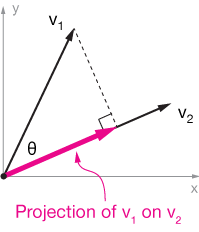
\includegraphics[width=.4\textwidth]{orthogonal-projection.png}}
    \caption{Geometrically, on the plane the projection of $\vec{v}$ over $\vec{w}$ is the vector whose final point is the intersection
between the line containing $\vec{w}$ and the line which is perpendicular to $\vec{w}$ containing the end point of $\vec{v}$.}
\end{figure}

Also, given the geometrical expression of the \nref{def:inner-product}, $\innerp{\vec{x}, \vec{y}} = \vnorm{\vec{x}}
\vnorm{\vec{y}}\cos(\theta)$, since $\abs{\cos(\theta)}\leq 1$, we deduce the following important result.
\begin{lemma}[Cauchy-Schwartz inequality]
$\forall\vec{x}, \vec{y}\in\Rtn \implies \abs{\innerp{\vec{x}, \vec{y}}}\leq \vnorm{\vec{x}}\vnorm{\vec{y}}$.
\end{lemma}

%\begin{proof}
%TODO.
%\end{proof}

\hide{
By making use of \ref{eq:inner-product} and \ref{def:euclidean-norm} we can now define the notion of angle between vectors.

\begin{defn}[Angle between vectors]
Given $\vec{v}$, $\vec{w}\in\Rtn$, the angle between the vectors $\vec{v}$ and $\vec{w}$ is the number $\theta\in[0, \pi]$ 
determined by the inner product as
\begin{equation}
\cos(\theta)_{\left(\vec{x}, \vec{y}\right)} = \frac{\innerp{\vec{x}, \vec{y}}}{\vnorm{\vec{x}}\vnorm{\vec{y}}}
\end{equation}
\end{defn}
}

\section{Set topology in $\Rtn$}

Topology is in charge of describing the different subsets of $\Rtn$ depending on the place that its points occupy. The
following are basic concepts of set topology and can be generalize to any metric space without defining explicitly the metric.

\begin{defn}[Open ball]
Given $\vec{x_0}\in\Rtn$ and a real number $\epsilon > 0$, an open ball with centered in $\vec{x_0}$ with radius $\epsilon$ is the set
\begin{equation}
B_\epsilon\argopen(\vec{x_0}\argclose)\bydef\{\vec{x}\in\Rtn\st\vnorm{\vec{x} - \vec{x_0}} < \epsilon\}.
\end{equation}
\end{defn}

\begin{note}
	In 2-dimensional space, balls are often called \textit{disks}.
\end{note}

\begin{defn}[Pierced open ball]
Given $\vec{x_0}\in\Rtn$ and a real number $\epsilon > 0$, a pierced open ball centered in $\vec{x_0}$ with radius $\epsilon$ is the
set $B'_\epsilon\argopen(\vec{x_0}\argclose)\bydef B_\epsilon\argopen(\vec{x_0}\argclose) - \{\vec{x_0}\}$. In other words, it's an 
open ball excluding its centre.
\end{defn}

\begin{defn}[Open set]
	A subset $S\subset\Rtn$ is called \textit{open} $\iff\forall\vec{x_0}\in S$ there exists $\epsilon > 0$ depending on $\vec{x_0}$ such that $B_\epsilon\argopen(\vec{x_0}\argclose)\subset S$. In other words, if $\forall\vec{x_0}\in S$ there exists $\epsilon > 0$
	such that a point in $\Rtn$ belongs to $S$ as soon as its Euclidean distance from $\vec{x_0}$ is smaller than $\epsilon$. 
\end{defn}

\begin{note}
An open set can be seen as a set that contains a ball around each of its points or, equivalently, a set which doesn't contain any of
its boundary points.
\end{note}

\begin{prop}
The union of infinitely many open sets and the intersection of a finite number of open sets are open.
\end{prop}

\begin{defn}[Closed set]
	A subset $S\subset\Rtn$ is called \textit{closed}, denoted by $\conj{S}$, if its complementary (relative to the space that it is defined on) $S^C \bydef\Rtn\setminus S$ is open. 
\end{defn}

\begin{prop}
The union of a finite number of closed sets and the intersection of infinitely many closed sets are closed.
\end{prop}

\begin{prop}
	The full space $\Rtn$ and null set $\O$ are both open and closed sets, known as \textit{clopen sets}.
\end{prop}

Open and closed sets generalize the idea of an open and closed interval in the real line to higher dimensions.

\begin{defn}[Interior]
	The interior of a subset $S\subset\Rtn$, denoted by $\interior{S}$, is the largest open subset of $\Rtn$ contained in $S$. 
	A point that is in the interior of $S$ is an \textbf{interior point}.
	\begin{equation}
		\interior{S}\bydef\{\vec{x_0}\in S\st\exists\epsilon > 0\implies B_\epsilon\argopen(\vec{x_0}\argclose)\subset S\}.
	\end{equation}
\end{defn}

\begin{defn}[Exterior]
	The exterior of a subset $S\subset\Rtn$, denoted by $\exterior{S}$, is the complementary set of the closure of $S$, defined as
	\begin{equation}
		\exterior{S}\bydef\{\vec{x_0}\in\Rtn\st\exists\epsilon > 0\implies B_\epsilon\argopen(\vec{x_0}\argclose)\subset
		\left(\Rtn\setminus S\right)\}.
	\end{equation}
	The points in this set are called \textbf{exterior points}.
\end{defn}

\begin{defn}[Closure]
	The closure of a subset $S\subset\Rtn$, denoted by $\closure{S}$, consists of all points in $S$ together with its boundary.
	Mathematically, 
	\begin{equation}
		\closure{S}\bydef\interior{S}\cup\frontier{S}.
	\end{equation}
	It is the smallest closed subset of $\Rtn$ contained in $S$, and its points are called \textbf{points of closure} of $S$.
\end{defn}

\begin{defn}[Boundary]
	The boundary, or frontier, of a subset $S\subset\Rtn$, denoted by $\frontier{S}$, is the set of points in the border of the
	set that can be approached both from $S$ and from the outside of $S$. More precisely, 
	\begin{equation}
		\frontier{S}\bydef\{\vec{x_0}\in\Rtn\st\exists\epsilon > 0\implies B_\epsilon
		\argopen(\vec{x_0}\argclose)\cap S\neq\O\land B_\epsilon\argopen(\vec{x_0}\argclose)\cap\left(\Rtn\setminus S\right)
		\neq\O\}.
	\end{equation}
	Equivalently, the boundary can be defined as $\frontier{S}\bydef\closure{S}\setminus\interior{S}$, and its points are called
	\textbf{boundary points}.
\end{defn}

\begin{prop}
	Let $S\subset\Rtn$, then the following properties hold:
	\begin{itemize}[itemsep = -2pt]
		\item $\interior{S}\cup\exterior{S}\cup\frontier{S} = \Rtn$.
		\item $\interior{S}\cap\exterior{S} = \interior{S}\cap\frontier{S} = \exterior{S}\cap\frontier{S} = \O$.
	\end{itemize}
\end{prop}

\begin{figure}[ht]
    \centering
    \incfig{open-ball}
    \caption{The black circle represents the set of points $(x, y)$ satisfying $x^2 + y^2 = \epsilon^2$, while the grey
    disk represents the set of points $(x, y)$ satisfying $x^2 + y^2 < \epsilon^2$. The grey set is an open set, the black
set is its boundary set and the union of both sets is a closed set, the closure.}
\end{figure}

\begin{defn}[Isolated point]
A point $\vec{x_0}$ of a subset $S\subset\Rtn$ is said to be isolated $\iff\forall\epsilon > 0, \exists B_\epsilon\argopen(\vec{x_0}
	\argclose)\st B_\epsilon\argopen(\vec{x_0}\argclose)\cap S = \{\vec{x_0}\}$.
\end{defn}

\begin{defn}[Limit point]
Given $S\subset\Rtn$, a point $\vec{x_0}\in S$ is said to be a limit point, or accumulation point, of $S\iff\forall\epsilon > 0, 
	\exists B'_\epsilon\argopen(\vec{x_0}\argclose)\st B'_\epsilon\argopen(\vec{x_0}\argclose)\cap S\neq\O$. In other words, 
	if we can find points of $S$ as much close as we want to the point $\vec{x_0}$.
\end{defn}

\begin{defn}[Bounded set]
A set $S\subset\Rtn$ is said to be \textit{bounded} $\iff\exists M > 0\st\forall\vec{x}\in S\implies \vnorm{\vec{x}}\leq M$.
\end{defn}

\begin{defn}[Compact set]
A set $S\subset\Rtn$ is said to be \textit{compact} if it's closed and bounded.
\end{defn}

\begin{defn}[Convex set]
A set is said to be \textit{convex} if when tracing a segment between any two points we don't get out of the set.
\end{defn}

%\section{Analytic geometry of lines and planes. Parametrization}
%We'll now study some objects in the Euclidean plane and space. In particular, lines in $\R^2$ and planes in $\R^3$.

\section{Functions of the form $\Rtn\longrightarrow\R^m$}
Now that we have defined $\Rtn$, we are interested in studying functions of the form $\stdvf$. Depending on the values of 
$n$ and $m$ we can distinguise between two kinds of functions.

\begin{defn}[Scalar-valued function]\label{def:scalar-function}
	A scalar-valued function over (a subset of) $\Rtn$ is a mapping $\appl{f}{S\subseteq\Rtn}{\R}$, $\left(x_1, \ldots, x_n\right)
	\longmapsto f\left(x_1, \ldots, x_n\right)$.
\end{defn}

\begin{defn}[Vector-valued function]
	A vector-valued function over $\Rtn$ is a mapping $\appl{f}{S\subseteq\Rtn}{\R^m}$, $\vec{x}\longmapsto\vec{y} = f(\vec{x})$, where
	if $f$ goes from $\Rtn$ to $\R^{m>1}$ then
	\begin{equation}
		\vec{y} = f(\vec{x})\bydef\begin{bmatrix}y_1 \\ \vdots \\ y_m \end{bmatrix} = \begin{bmatrix}f_1(x_1, \ldots, x_n) \\
		\vdots \\ f_m(x_1, \ldots, x_n)\end{bmatrix}.
	\end{equation}
\end{defn}

\begin{remark}
	A vector function $\appl{f}{S\subseteq\Rtn}{\R^m}$ is given by $m$ scalar functions $\appl{f_i}{\Rtn}{\R}$ with $i = 1, \ldots,
	m$, where $f_i(x_1, \ldots, x_n)$ gives us the $i$-th component of $f$.
\end{remark}

\begin{example}
    The following function of several variables $f(x, y, z) = x + y + 2z$ is a scalar function.
\end{example}

% These are just the classical domain, image, etc., but extended to functions of several variables in $\Rtn$.

\begin{defn}[Domain]
Given a function $\stdvf$, the \textit{domain} of that function is the set of points in $\Rtn$ for which the function $f$ is 
defined, in other words, the set
\begin{equation}
\dom{f} \bydef \{\vec{x}\in\Rtn\st\exists f(\vec{x})\}\subseteq\Rtn.
\end{equation}
\end{defn}

\noindent For vector-valued functions; i.e. functions of the form $\stdvf$ with $m > 1$, the overall domain is the intersection of the
domains of each function defining $f$,
\begin{equation}
\dom{f}\bydef\bigcap_{i=1}^m\altdom{f_i}.
\end{equation}

\begin{defn}[Image]
Given a function $\stdvf$, the \textit{image} or \textit{range} of $f$ is the set
\begin{equation}
\image{f}\bydef\{\vec{y}\in\R^m\st \vec{y} = f\left(\vec{x}\right),\ \forall\vec{x}\in\altdom{f}\}\subseteq\R^m.
\end{equation}
\end{defn}

\begin{defn}[Graph]
Given a vector-valued function $\stdvf$, the graph of $f$ is the set
\begin{equation}
\fgraph{f}\bydef\{\left(\vec{x}, f\left(\vec{x}\right)\right)\st\vec{x}\in\altdom{f}\}\subset\R^{n + m}.
\end{equation}
\end{defn}

For $n\geq 3$ it's pretty difficult (actually, we can't) to draw graphs of functions. Nevertheless, this graphs
can be drawn using the concept of level sets.

\begin{defn}[Level sets]
Given a function $\gmvf$ and a scalar $c\in\R$, the level set of value $c$ for the function $f$ is a subset of the initial space
defined as
\begin{equation}
\levelset{c}{f} \bydef \{\vec{x}\in\altdom{f}\st f\left(\vec{x}\right) = c\}\subset\Rtn.
\end{equation}
\end{defn}

\begin{note}
    For $n=2$, this sets are called \textbf{level curves}, and for $n=3$, \textbf{level surfaces}.
\end{note}

Let us consider the graph of $\appl{f}{\R^2}{\R}$. Take its intersection with the plane $z = c$. This intersection gives 
us a curve in the initial space. This curve of level $c$ of $f$ is obtained by projecting the space curve onto the $XY$
plane.

\begin{example}
    Let $\appl{f}{\R^2}{\R}, (x, y)\longmapsto x^2 + y^2$. The level curve of level $c\geq 0$ of $f$ is a circle of radius
    $\sqrt{c}$ centered at the origin. The graph of $f$ is a surface called \textit{circular paraboloid}, which is obtained
    by rotating a parabola about its symmetry axis.
\end{example}

\begin{example}
    Let $\appl{f}{\R^2}{\R}, (x, y)\longmapsto x^2 - y^2$. When $c\neq 0$ we have a curve with equation $y = \pm\sqrt{x^2 - c}$.
    For $c > 0$, its level curve is a hyperbola in the region $\{(x, y)\st \abs{y} < x\}$. For $c < 0$, it is a hyperbola in
    $\{(x, y)\st\abs{y} > x\}$. Finally, when $c = 0$, we have the curve $y = \pm x$. In this case, the graph of $f$ is a 
    surface called \textit{hyperbolic paraboloid}.
\end{example}

\begin{example}
    Let $\appl{f}{\R^2}{\R}, (x, y)\longmapsto x^2 + 4y^2$. For each $c\geq 0$, the curve of level $c$ is an ellipse with
    equation $x^2 + 4y^2 = c$. Since $f > 0, \forall x, y\in\R$, for $c < 0$ the curve is the empty set. The graph of $f$ is
    a surface called \textit{elliptic paraboloid}.
\end{example}

\begin{remark}
    In functions of the form $f(x, y) = a_1x^2 + a_2y^2 + a_3$ with fixed coefficients $a_i\in\R$ and $a_1, a_2$ nonzero, the
    graphs can be classified as follows.
    \begin{itemize}[itemsep = -2pt]
        \item If $a_1, a_2$ have the same sign the graph of $f$ is an elliptic paraboloid. If $a_1 = a_2$, the graph is a 
            circular paraboloid.
        \item If $a_1, a_2$ have different sign the graph of $f$ is a hyperboloid paraboloid.
    \end{itemize}
\end{remark}

\section{Limits in $\Rtn$. Convergence of sequences and continuous functions}

\section{Topological properties of continuous functions}
